\ifdefined\namedversion
\documentclass[12pt]{clear2027}
\else
\documentclass[anon,12pt]{clear2027}
\fi
\usepackage[T1]{fontenc}
\usepackage{times,booktabs,mathtools}
\emergencystretch=3em
\newcommand{\E}{\mathbb{E}}
\newcommand{\Prb}{\mathbb{P}}
\newcommand{\Var}{\operatorname{Var}}
\newcommand{\ind}{\mathbf{1}}
\newcommand{\calS}{\mathcal{S}}
\newcommand{\calQ}{\mathcal{Q}}
\title[Winner Logs and Counterfactual Audits]{What Winner Logs Cannot Tell You:\\Counterfactual Audits of First-Response Systems}
\clearauthor{\Name{Shivam Gupta} \Email{shivam20406@iiitd.ac.in}\\\addr Independent Researcher}
\ifdefined\namedversion
\jmlrvolume{}\jmlryear{2026}\jmlrproceedings{Research manuscript}{Research manuscript}\editor{}
\fi
\begin{document}
\maketitle
\begin{abstract}
Parallel inference systems often return the first response and cancel the rest. Their logs then conceal the responses required to evaluate alternative endpoint-exclusion policies. We study response-suppression interventions that preserve the surviving response mechanisms, allowing arbitrary dependence between endpoint quality and completion time. A prefix of depth $r+1$ is universally sufficient, and necessary among deterministic prefix logs, to evaluate every exclusion of at most $r$ endpoints. Randomized retention identifies these effects through standard inverse-inclusion weighting. Our main results characterize the information needed to allocate this audit: given only winner probabilities and binary rewards, uniform retention is exactly minimax for audit-induced variance within rank-only prefix designs. Exchangeable completion orders instead admit a decreasing square-root allocation. Two systems with identical winner logs have different optimal allocations; transferring the exchangeable allocation to a paired-order system incurs an exact variance ratio $\sqrt{m-2}$ at one extra retained response per request. We provide a monotone allocation solver with primal--dual checks, complete proofs, and reproducible experiments. Across six trained classifiers, three public datasets, ten splits, and engineered latency environments, pilot optimization offers modest median gains but can fail badly on sparse calibration data. The results establish an observability requirement and a conditional evaluation method, rather than a guarantee for physical outages or load-changing interventions.
\end{abstract}
\begin{keywords}
causal evaluation, response suppression, competing risks, randomized auditing, parallel inference
\end{keywords}

\section{Introduction}
An inference gateway may send one request to several models, accept the first valid response, and cancel the remaining calls. This can reduce latency, but it also determines what the operator can learn. A log containing the winning endpoint, its answer, and its completion time does not generally reveal the answer that would have been selected had that endpoint been excluded. Such comparisons matter when an operator considers excluding a provider, restricting a model family, or changing which parallel responses are eligible to serve a request.

The general statistical problem of learning from cancelled runs is established. Hedged requests are a standard tail-latency technique \citep{dean2013}; censored runtime data arise in algorithm portfolios \citep{gagliolo2007,hutter2014}; and competing-risk observations need not identify latent alternatives \citep{tsiatis1975}. The question here is more specific: how much additional observation is required to evaluate a \emph{whole menu} of response-exclusion interventions, and what can the original winner logs tell us about how to allocate that observation?

We study a structural intervention on response eligibility. Every endpoint has a completion time and a scored response, possibly dependent on all the other endpoints through shared request difficulty or common exogenous variables. Excluding an endpoint changes which completed response is selected, while preserving these potential times and responses. This intervention is directly implementable by suppressing responses at a collector. It also represents an endpoint's physical removal only under an additional mechanism-invariance assumption. We explicitly distinguish these interpretations.

A small amount of structured observation can support many comparisons. If at most $r$ endpoints can be excluded, the first surviving response must occur among the first $r+1$ completions. A single retained prefix therefore serves $\sum_{k=1}^r\binom{m}{k}$ policies. However, ``retain a prefix'' does not specify a good audit. A design that usually retains only the second response can be efficient if the first surviving response is usually second, yet extremely poor when informative policies require the third response.

Our main contribution is a sharp distinction between information available in winner logs and information needed for audit allocation. Among rank-only randomized prefix designs, winner probabilities alone justify uniform retention as the exact worst-case choice. Knowing that completion order is exchangeable justifies a different square-root schedule. These conclusions cannot be distinguished using winner logs: we construct systems with identical first responses for which transferring the exchangeable schedule incurs an unbounded approximation ratio as the number of endpoints grows. This is a statement about audit geometry, not about a new inverse-probability estimator.

We also give a finite-cohort evaluation workflow with exact audit variance, a monotone convex allocation and a checkable dual bound. Experiments deliberately retain negative results: learning the allocation from a small pilot is fragile, and ordinary normal intervals can be unreliable for rare effects. The application is relevant to parallel model gateways and speculative tool services, but the empirical evidence uses trained classifiers with engineered latencies, not commercial LLM traffic.

\begin{figure}[t]
\centering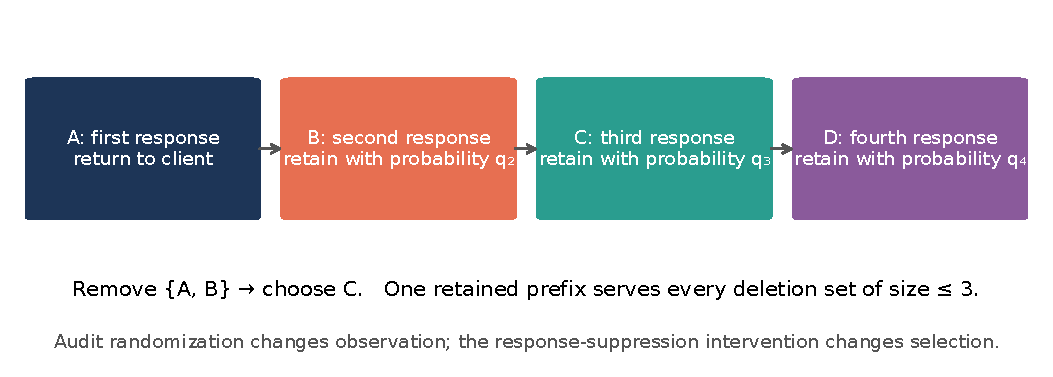
\includegraphics[width=\linewidth]{../figures/prefix.pdf}
\caption{One completion prefix supports many response-suppression interventions. The client's first response is released immediately; a separate randomized audit controls which later responses are retained. Suppression changes selection, whereas audit randomization changes observation.}
\label{fig:prefix}
\end{figure}

\section{Related Work and the Scope of the Contribution}
\paragraph{Parallel execution and censoring.}
\citet{dean2013} describe hedging and cancellation as tail-tolerance mechanisms. \citet{gagliolo2007} learn runtime distributions during parallel algorithm execution, and \citet{hutter2014} discuss censored observations in runtime prediction. We do not claim that cancellation-induced missingness is new. Our targets are quality contrasts for a fixed menu of endpoint suppressions, rather than runtime prediction or online allocation of solver time. Correlation between quality and completion time is unrestricted.

\paragraph{Competing risks and intervention semantics.}
\citet{tsiatis1975} establish nonidentifiability in competing-risk models. Our prefix-depth obstruction is a finite response-table instance of a missing-alternative problem, not a replacement for that theory. The proposed audit changes the observation process prospectively, giving known inclusion probabilities. Importantly, observing additional alternatives does not identify how their mechanisms would change under a different load or launch policy.

\paragraph{Unequal-probability sampling and randomized truncation.}
The inverse-inclusion estimator is a Horvitz--Thompson construction \citep{horvitz1952}, related to inverse-probability methods for missing data \citep{robins1994}. Randomly retaining a computational prefix is closely related to Russian roulette and randomized telescoping \citep{lyne2015,beatson2019}; optimal truncation distributions are studied by \citet{cui2021}. Square-root allocation, convex multivariate allocation \citep{bethel1989}, and pooling adjacent order violations are established tools. We claim neither the weighting identity nor these optimization principles as new. The specific contributions are the response-suppression reduction, sharp winner-information and exchangeability envelopes, and the indistinguishable-system separation, together with their implementation and empirical boundaries.

\paragraph{Partial monitoring and direct policy comparisons.}
Cascading bandits observe a prefix determined by the first attractive item and optimize online ranking \citep{kveton2015}. Here a latency order determines response selection, rewards may be arbitrarily dependent, and the design controls additional observation after selection. Direct policy comparison can remove uncertainty in regions where policies agree \citep{guerdan2024}; our contrast is exactly zero whenever the baseline winner is not excluded. The resulting audit is not a general solution to confounded off-policy evaluation.

\section{Response-Suppression Model}
For one request, let $U$ contain all exogenous variables, including task difficulty, endpoint randomness and common disturbances. Endpoint $a\in[m]$ has time $T_a=t_a(U)$ and quality $Y_a=y_a(U)\in[0,1]$. All endpoints are launched under a fixed protocol. Times are finite; ties use a fixed deterministic endpoint priority. Write $\pi=(\pi_1,\ldots,\pi_m)$ for the resulting completion order, and $Y_{(j)}=Y_{\pi_j}$. No endpoint independence is assumed.

For $S\subset[m]$, suppress responses from endpoints in $S$ at the selector. Define
\begin{equation}
 J_S=\min\{j:\pi_j\notin S\},\qquad
 D_S=Y_{(J_S)}-Y_{(1)}.\label{eq:target}
\end{equation}
The target menu is $\calS_r=\{S:1\le |S|\le r\}$ for $r<m$. For a fixed cohort $\mathcal F=(F_1,\ldots,F_n)$ of full response tables, the estimand is
\begin{equation}
 \theta_S=\frac1n\sum_{i=1}^n D_{iS}.\label{eq:cohort}
\end{equation}
This is a causal contrast under the structural selector intervention just defined. Inference below conditions on the cohort; the randomness is the prospective audit. Generalizing to a population additionally requires a sampling argument.

\paragraph{Observation versus intervention.}
Ordinary cancellation records only $(\pi_1,T_{(1)},Y_{(1)})$. A prefix audit retains completions through a random rank $R\le r+1$, with cumulative inclusion probabilities
\begin{equation}
 q_1=1\ge q_2\ge\cdots\ge q_{r+1}>0,\qquad
 \Prb(R\ge j\mid F)=q_j.\label{eq:q}
\end{equation}
A rank-only design chooses $R$ independently of the full response table; draw $V\sim\mathrm{Uniform}(0,1)$ and retain exactly the ranks with $V<q_j$. Independent draws are used across requests. The audit may run after the client receives the first response. Endpoint completion quality is scored by a declared evaluator. If scoring is itself unavailable for retained responses, an additional missing-label problem remains.

\paragraph{Physical removal is a stronger claim.}
Suppression preserves $t_a,y_a$ by definition. Removing a provider before launch, changing routing, or changing cancellation policy can alter shared queues, model state, or resource contention. Equation~\eqref{eq:target} represents those interventions only if surviving response mechanisms are invariant. Our results do not infer that invariance from winner logs.

\section{Identification and Exact Audit Risk}
\begin{theorem}[Universal prefix depth]\label{thm:depth}
The first $r+1$ endpoint identities and rewards determine $D_S$ for every $S\in\calS_r$. No deterministic prefix depth $d\le r$ universally identifies all these contrasts over unrestricted response tables. For randomized prefixes, positive inclusion through rank $r+1$ suffices for point identification; if inclusion vanishes at an attainable required rank, universal identification fails.
\end{theorem}
\begin{proof}
Among $r+1$ distinct identities, at least one survives $S$. Hence $J_S\le r+1$ and its reward is observed. Conversely, fix a logged prefix of depth $d\le r$ and choose $S$ to contain that prefix. Two full tables can agree on every logged identity, time and reward but assign different rewards to the first unlogged survivor. The contrast then differs. The same two-world construction applies to a zero-inclusion rank. Positive inclusion identifies the contrast by Theorem~\ref{thm:ht}.
\end{proof}

\begin{theorem}[Inverse-inclusion evaluation]\label{thm:ht}
For a logged prefix, let $Z_S$ be zero if the prefix contains no surviving endpoint; otherwise let $j$ be the first surviving rank and set $Z_S=(Y_{(j)}-Y_{(1)})/q_j$. Then
\begin{align}
 \E[Z_S\mid F]&=D_S,\label{eq:ht}\\
 \Var(Z_S\mid F)&=D_S^2(q_{J_S}^{-1}-1).\label{eq:var}
\end{align}
With independent audit draws, $\widehat\theta_S=n^{-1}\sum_i Z_{iS}$ is conditionally unbiased and
\begin{equation}
 n\Var(\widehat\theta_S\mid\mathcal F)
 =\sum_{j=2}^{r+1}A_{Sj}(q_j^{-1}-1),\quad
 A_{Sj}=\frac1n\sum_i\ind\{J_{iS}=j\}D_{iS}^2.\label{eq:A}
\end{equation}
\end{theorem}
\begin{proof}
For a fixed full table, the computable statistic is $Z_S=\ind\{R\ge J_S\}D_S/q_{J_S}$. Its first two conditional moments are $D_S$ and $D_S^2/q_{J_S}$. Sum independent row variances. Rank one contributes zero because $D_S=0$ whenever $J_S=1$.
\end{proof}

The estimator uses only a revealed prefix and its propensities. It never reads the hidden order to decide whether a censored row contributes zero. Complete-case analysis is different: discarding unresolved rows changes the target cohort and generally biases the contrast.

\paragraph{Finite-sample statements.}
If $q_j\ge\delta>0$, Hoeffding's inequality and a union bound imply, conditionally on any fixed cohort,
\begin{equation}
 \Prb\!\left(\max_{S\in\calS_r}|\widehat\theta_S-\theta_S|>
 \frac1\delta\sqrt{\frac{\log(2|\calS_r|/\alpha)}{2n}}\ \middle|\ \mathcal F\right)\le\alpha.\label{eq:hoeffding}
\end{equation}
For each fixed row and target, $Z_{iS}$ takes values in an interval of length at most $1/\delta$, even though its sign may differ across rows. The bound can be conservative. An unbiased estimator of conditional audit variance is
\begin{equation}
 \widehat V_S=\frac1{n^2}\sum_{i:\,R_i\ge J_{iS}}
 D_{iS}^2\frac{1-q_{J_{iS}}}{q_{J_{iS}}^2}.\label{eq:vhat}
\end{equation}
Using $1.96\sqrt{\widehat V_S}$ is only an asymptotic approximation; our experiments expose undercoverage for sparse contrasts.

\section{What Winner Logs Can and Cannot Justify}
We now compare designs before collecting a cohort. The loss is the expected \emph{audit-induced} variance, not the full sampling variance of a population effect estimator:
\begin{equation}
 \mathcal R_P(q)=\max_{S\in\calS_r}\E_{F\sim P}\!\left[D_S^2(q_{J_S}^{-1}-1)\right].\label{eq:risk}
\end{equation}
For $n$ independent full tables, this is $n$ times the maximum expected conditional variance in Equation~\eqref{eq:A}. It excludes variation of the full-table effect across independently sampled requests. Consider an expected completion budget $0<b\le r$:
\begin{equation}
 \calQ_b=\left\{1\ge q_2\ge\cdots\ge q_{r+1}>0:
 \sum_{j=2}^{r+1}q_j\le b\right\}.\label{eq:budget}
\end{equation}
The sum is the expected number of additional \emph{retained completions}. It is not generally an API bill or a wall-time budget.

\begin{theorem}[Sharp winner-only guarantee]\label{thm:winner}
Suppose rewards are binary and the winner-only law is known, including winner identity probabilities $p_a$. Let $\mathcal P(p)$ be all full-table laws compatible with that winner-only law, and let $\gamma_r(p)$ be the sum of its $r$ largest identity probabilities. Then for every $q\in\calQ_b$,
\begin{equation}
 \sup_{P\in\mathcal P(p)}\mathcal R_P(q)
 =\gamma_r(p)(q_{r+1}^{-1}-1).\label{eq:winner}
\end{equation}
Consequently,
\begin{equation}
 \inf_{q\in\calQ_b}\sup_{P\in\mathcal P(p)}\mathcal R_P(q)
 =\gamma_r(p)(r/b-1),\label{eq:minimax}
\end{equation}
attained by $q_2=\cdots=q_{r+1}=b/r$.
\end{theorem}
\begin{proof}
A nonzero contrast requires $\pi_1\in S$. Since $D_S^2\le1$ and the reciprocal inclusion penalty increases with rank,
$\E[D_S^2(q_{J_S}^{-1}-1)]\le\Prb(\pi_1\in S)(q_{r+1}^{-1}-1)\le\gamma_r(p)(q_{r+1}^{-1}-1)$.
For equality, choose $S$ as the $r$ most probable winner identities. Conditional on a winner in $S$, put the other $r-1$ identities of $S$ next, then any survivor. Give that survivor the opposite binary reward to the winner. Preserve the given winner identity, time and reward on every request; choose later times strictly increasing. This produces a compatible full-table law attaining the bound. Finally, monotonicity and the budget imply $rq_{r+1}\le b$. Uniform retention attains the largest feasible final inclusion probability.
\end{proof}

This is a minimax result \emph{within rank-only prefix designs using the estimator above}. It is not a lower bound over all estimators, response-specific audits, or experiments that randomize which endpoints are launched. Winner-only logs support a robust design, but they do not establish exchangeability of the hidden ordering.

\begin{theorem}[Exchangeable-order envelope]\label{thm:exch}
Suppose the endpoint order is uniform over all permutations, while rewards conditional on order remain arbitrary in $[0,1]$. Then
\begin{equation}
 \sup_P\mathcal R_P(q)=\sum_{j=2}^{r+1}p_j^{(m,r)}(q_j^{-1}-1),\qquad
 p_j^{(m,r)}=\frac{(r)_{j-1}(m-r)}{(m)_j},\label{eq:exch}
\end{equation}
where $(x)_k=x(x-1)\cdots(x-k+1)$. For unit completion costs, the minimizing design is
\begin{equation}
 q_j=\min\{1,\kappa\sqrt{p_j^{(m,r)}}\},\quad
 \sum_{j=2}^{r+1}q_j=b.\label{eq:sqrt}
\end{equation}
\end{theorem}
\begin{proof}
For $|S|=r$, the event $J_S=j$ requires the first $j-1$ identities to lie in $S$ and the next outside it; its probability is Equation~\eqref{eq:exch}. Bounding $D_S^2$ by one gives the envelope. Assign the winner reward zero and every later reward one to attain it simultaneously for all $S$. Smaller exclusion sets have stochastically smaller first-survivor rank and hence no larger loss. The coefficients decrease with $j$, since $p_{j+1}/p_j=(r-j+1)/(m-j)\le1$. The budget-constrained separable convex problem has the clipped square-root solution, which already satisfies the order restriction.
\end{proof}

\begin{theorem}[Indistinguishable winner logs, divergent allocations]\label{thm:twins}
Let $m\ge4$ be even, $r=2$, and $b=1$. There exist two response-table laws with identical winner identities, winner times and winner rewards. Under the first law the optimal rank-only design is
\begin{equation}
 (q_2,q_3)=\frac{(\sqrt{m-2},1)}{\sqrt{m-2}+1}.\label{eq:twinq}
\end{equation}
Under the second law the unique optimal design is $(1/2,1/2)$. Applying Equation~\eqref{eq:twinq} to the second law gives the exact variance ratio
\begin{equation}
 \frac{\mathcal R_{\rm paired}(q^{\rm exchangeable})}
 {\inf_{q\in\calQ_1}\mathcal R_{\rm paired}(q)}=\sqrt{m-2}.\label{eq:ratio}
\end{equation}
\end{theorem}
\begin{proof}
In both laws the winner is uniform on $[m]$, its time is one, its reward is zero, later times are $2,\ldots,m$, and all later rewards are one. The first law draws a uniform permutation. Theorem~\ref{thm:exch} gives $p_2=2(m-2)/(m(m-1))$, $p_3=2/(m(m-1))$, yielding Equation~\eqref{eq:twinq}.
For the second law partition the endpoints into pairs. Given the uniform winner, place its partner second and all remaining endpoints afterwards in any fixed order. Suppressing a pair makes $J_S=3$ with probability $2/m$; suppressing a nonpair of size two makes $J_S=2$ with probability $2/m$. Singletons have probability $1/m$ of requiring rank two. Since $q_3\le q_2$, the worst loss is $\mathcal R_{\rm paired}(q)=(2/m)(1/q_3-1)$. Its unique optimum has $q_2=q_3=1/2$, with loss $2/m$. Substitution gives Equation~\eqref{eq:ratio}.
\end{proof}

\begin{figure}[t]
\centering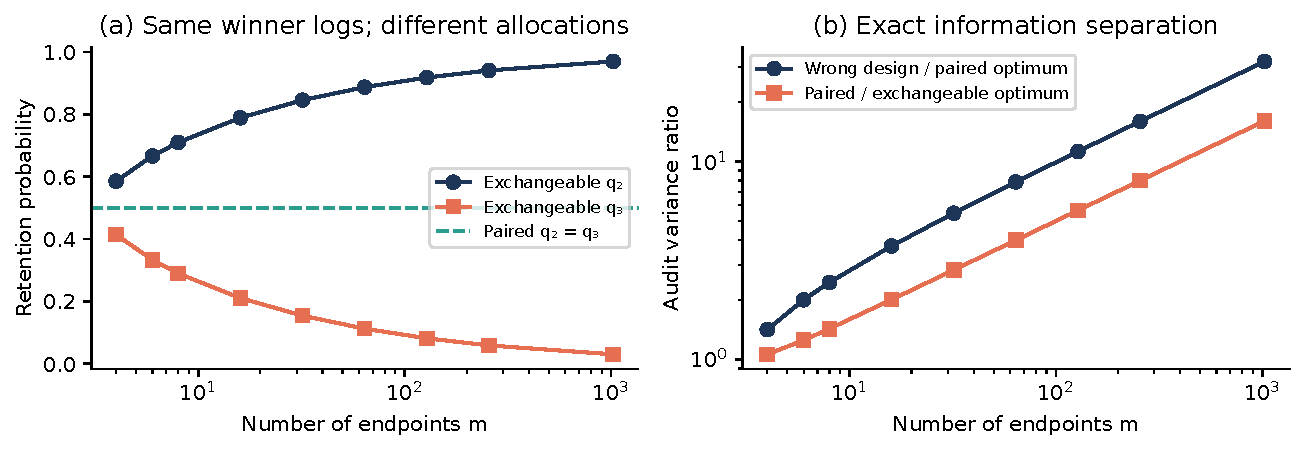
\includegraphics[width=\linewidth]{../figures/twins.pdf}
\caption{Exact separation for systems with identical winner logs ($r=2$, $b=1$). The exchangeable design increasingly favors rank two; the paired system requires equal inclusion at ranks two and three. The wrong-design ratio is exactly $\sqrt{m-2}$. The second ratio compares the two systems' optimal risks. Curves are theorem calculations, not measured provider data.}
\label{fig:twins}
\end{figure}

The separation isolates an actionable question: which endpoints tend to complete \emph{together before the first survivor}? Winner frequencies do not answer it. In the paired law, uniform retention is robustly justified by Theorem~\ref{thm:winner}; in the exchangeable law, additional order information permits a better allocation. At $m=1024$, transferring the exchangeable design increases paired-system variance by $31.97$ times. This does not mean 1024 production models were tested.

\section{Allocation with Richer Pilot Data}
A fully observed pilot can estimate the coefficients $A_{Sj}$ in Equation~\eqref{eq:A}. For a specified coefficient matrix, expected incremental costs $c_j>0$, and a positivity floor $\delta$, consider
\begin{equation}
 \min_{q\in\mathcal Q(b,c,\delta)}\max_{S\in\calS_r}
 f_S(q),\qquad f_S(q)=\sum_{j=2}^{r+1}A_{Sj}(1/q_j-1),\label{eq:opt}
\end{equation}
where $\mathcal Q(b,c,\delta)$ enforces $1\ge q_2\ge\cdots\ge q_{r+1}\ge\delta$ and $\sum c_jq_j\le b$. This is a convex program. The pilot is separate from evaluation; its optimizer is not guaranteed to optimize the evaluation cohort.

\paragraph{A numerical certificate.}
For any nonnegative target weights $\lambda_S$ summing to one,
\begin{equation}
 L(\lambda)=\min_{q\in\mathcal Q}\sum_S\lambda_S f_S(q)
 \ \le\ \min_{q\in\mathcal Q}\max_S f_S(q).\label{eq:dual}
\end{equation}
A feasible $q$ gives upper bound $U(q)=\max_S f_S(q)$. Thus $U(q)-L(\lambda)$ is a checkable gap. Compactness and convexity give equality after maximizing $L$ over the simplex. For the inner problem set $a_j=\sum_S\lambda_S A_{Sj}$. Pool adjacent ranks whose ratios $a_j/c_j$ violate decreasing order. A pooled block $B$ has a common inclusion probability
\begin{equation}
 q_B=\operatorname{clip}_{[\delta,1]}\!\left(
 \kappa\sqrt{\frac{\sum_{j\in B}a_j}{\sum_{j\in B}c_j}}\right).\label{eq:pava}
\end{equation}
Choose $\kappa$ by scalar budget search. Appendix~\ref{app:opt} derives the pooling rule. The software maximizes the dual with SLSQP, checks feasibility, and uses an independent primal epigraph solve when needed. Numerical gaps are floating-point bounds checked against another solve, not interval-arithmetic certificates.

\paragraph{Costs beyond retained completions.}
Let $\Delta T_j=T_{(j)}-T_{(j-1)}$. For rank-only retention,
\begin{align}
 \E[T_{(R)}-T_{(1)}]&=\sum_{j=2}^{r+1}q_j\E[\Delta T_j],\label{eq:wall}\\
 \E[\text{extra active endpoint time}]&=
 \sum_{j=2}^{r+1}q_j(m-j+1)\E[\Delta T_j].\label{eq:active}
\end{align}
The second identity assumes every unfinished endpoint remains active until audit termination and cancellation stops its accounted work immediately. In each intercompletion interval exactly $m-j+1$ endpoints remain unfinished. These identities permit wall-time or active-time coefficients in Equation~\eqref{eq:opt}. Real billing rules, uncancellable calls and delayed cancellation require their own cost model. A small completion budget alone does not establish small compute cost.

\paragraph{Pilot uncertainty.}
If $|\widehat A_{Sj}-A_{Sj}|\le\epsilon_j$ uniformly, then the regret of a pilot minimizer relative to the oracle over the same feasible set is at most
\begin{equation}
 2\sup_{q\in\mathcal Q}\sum_j\epsilon_j(1/q_j-1)
 \le2(\delta^{-1}-1)\sum_j\epsilon_j.\label{eq:regret}
\end{equation}
This follows by applying the uniform objective error at the two minimizers. A floor protects identification, but a small floor can still allow large variance when a rare informative rank is absent from the pilot. Our negative-transfer experiment is an example of this distinction.

\section{Reproducible Evaluation}
\paragraph{Protocol and datasets.}
The primary protocol was saved before model fitting and audit simulation. We use the bundled digits, Wisconsin diagnostic breast cancer and wine datasets \citep{datasets,pedregosa2011}. Stratified train/pilot/evaluation fractions are $0.50/0.20/0.30$, with split seeds $100$--$109$. Evaluation sizes are respectively $540$, $171$, and $54$. Six frozen classifiers are Gaussian naive Bayes, standardized logistic regression, random forest, extra trees, standardized 5-nearest neighbors, and standardized SVC. Forests have 80 trees; other settings and version pins are given in Appendix~\ref{app:exp}. In total 180 models are fitted. Pilot outcomes alone determine operational allocations.

\paragraph{Latency environments.}
The predictions are measured model outputs; completion times are \emph{engineered}, not measured provider runtimes. We test exchangeable exponential times, heterogeneous lognormal times with a shared request factor, and a correctness-correlated variant that makes correct responses slower. This separation permits exact full-table evaluation under controlled dependence. It does not establish the prevalence of such dependence in LLM gateways. The asynchronous runtime test separately checks execution, early winner release and loser cancellation using controlled service delays.

\paragraph{Targets, designs and loss.}
There are $m=6$ endpoints, $r=3$, and 41 prespecified exclusion targets. Budgets are $b\in\{0.25,0.5,1,2\}$ extra retained completions per request. We compare uniform retention, a geometric schedule, the exchangeable envelope schedule, pilot optimization, and an evaluation-cohort oracle shown only as a diagnostic. All optimized designs enforce $q_j\ge0.005$. The primary loss is exact worst-target conditional audit variance from Equation~\eqref{eq:A}; it has no Monte Carlo estimation error once the full table is fixed. The study includes 360 dataset, split, environment and budget conditions and 1800 design evaluations. All conditions are retained.

\begin{table}[t]
\centering\small
\caption{Median percentage reduction in exact worst-target audit variance relative to uniform retention at $b=0.5$. Parentheses count splits with higher variance than uniform. Each row includes all ten splits. Positive is better. The oracle uses held-out rewards and is not an operational method.}
\label{tab:results}
\begin{tabular}{llrrr}\toprule
Dataset & Latency & Exchangeable & Pilot & Oracle\\\midrule
digits & exponential & 5.4 (1/10) & 5.9 (1/10) & 8.5 (0/10) \\
digits & heterogeneous & -2.5 (6/10) & 3.2 (1/10) & 4.6 (0/10) \\
digits & correlated & -5.0 (7/10) & 3.7 (1/10) & 4.6 (0/10) \\
breast cancer & exponential & 9.1 (4/10) & 4.1 (4/10) & 11.8 (0/10) \\
breast cancer & heterogeneous & -5.0 (6/10) & 0.5 (4/10) & 3.4 (0/10) \\
breast cancer & correlated & -15.9 (9/10) & -2.4 (6/10) & 1.5 (0/10) \\
wine & exponential & -2.6 (5/10) & -0.0 (2/10) & 15.6 (0/10) \\
wine & heterogeneous & -0.2 (5/10) & 0.0 (1/10) & 13.2 (0/10) \\
wine & correlated & -25.9 (6/10) & 1.0 (3/10) & 3.4 (0/10) \\

\bottomrule\end{tabular}
\end{table}

\paragraph{Allocation results.}
Table~\ref{tab:results} and Figure~\ref{fig:empirical} show modest median benefits rather than a uniform improvement. For digits, pilot optimization reduces worst-target variance by median $5.9\%$, $3.2\%$, and $3.7\%$ in the three environments at $b=0.5$. On breast cancer with correctness-correlated times, the median change is a $2.4\%$ increase. The most severe pilot failure in the budget-$0.5$ comparison is a $1920.4\%$ increase in the heterogeneous wine environment: the small pilot misses a rank needed by a held-out contrast and assigns it the positivity floor. This is an informative failure, not a reason to discard the split. Geometric retention is worse than uniform in 88 of the 90 budget-$0.5$ conditions. The known exchangeable order law does not guarantee empirical optimality when rewards vary with rank and endpoint.

\begin{figure}[t]
\centering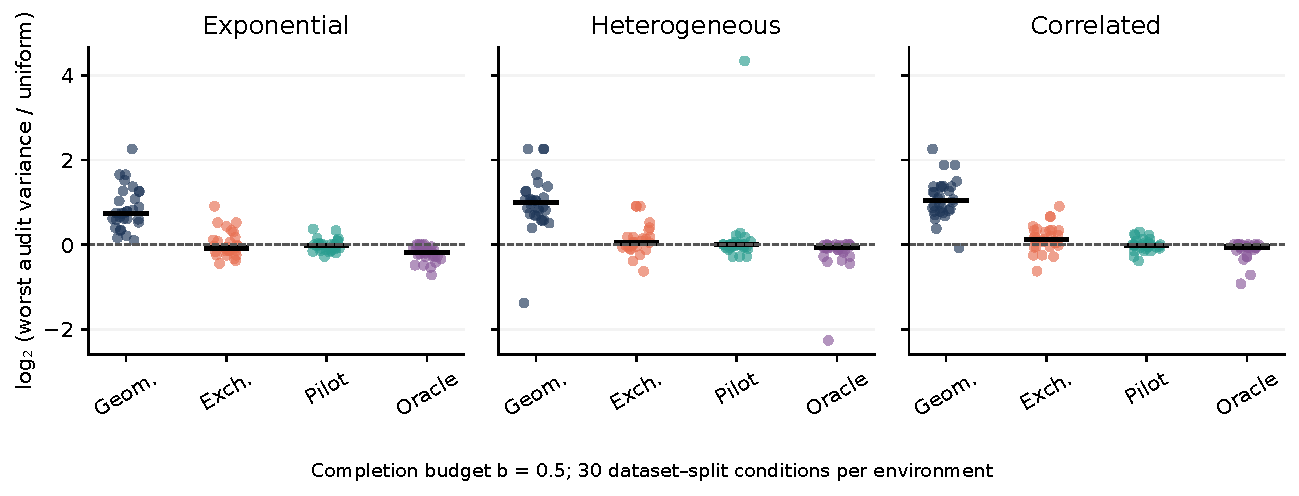
\includegraphics[width=\linewidth]{../figures/empirical.pdf}
\caption{All 90 dataset, split and environment conditions at $b=0.5$. Points give log variance ratios to uniform; black bars are medians. Values above zero are worse. The oracle isolates available allocation benefit; pilot and exchangeable schedules can lose on evaluation data. No outliers are removed.}
\label{fig:empirical}
\end{figure}

\paragraph{Unbiasedness, bias and intervals.}
For seed 100 we run 500 independent audit repetitions per dataset/environment, sharing uniform draws across designs. In the digits/exponential condition, uniform retention has worst-target exact standard deviation $0.02230$ and observed worst-target RMSE $0.02207$. Its maximum absolute Monte Carlo bias is $0.00119$, versus $0.03040$ for complete-case analysis. These numerical checks support the exact moment identity; they are not a substitute for its proof. Figure~\ref{fig:bias} illustrates the complete-case shift on digits/heterogeneous traces. The minimum targetwise coverage of ordinary 95\% normal intervals in the digits/exponential condition is only $41.0\%$ for uniform retention. Sparse nonzero contrasts can produce a zero estimated variance when their informative rows are not retained. Equation~\eqref{eq:hoeffding}, rather than the normal approximation, is our finite-sample guarantee.

\begin{figure}[t]
\centering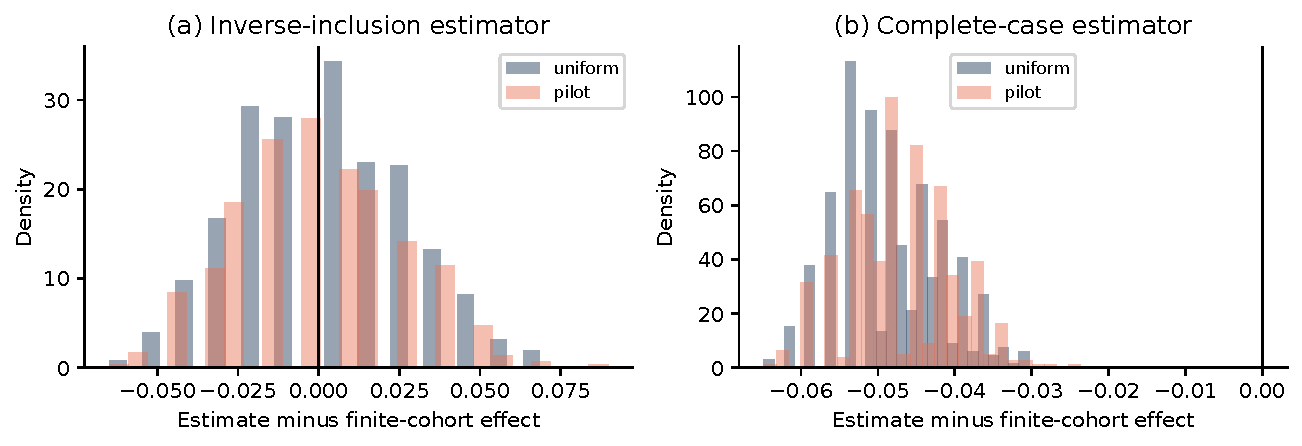
\includegraphics[width=\linewidth]{../figures/bias.pdf}
\caption{Audit repetitions on digits with heterogeneous engineered latencies, $b=0.5$, seed 100. For each displayed design, the target maximizes its absolute complete-case bias across the 41 prespecified targets. This diagnostic selection is used only to illustrate bias, not for a hypothesis test. Left: inverse-inclusion estimates. Right: complete-case estimates. The vertical line denotes zero error relative to the full-cohort effect.}
\label{fig:bias}
\end{figure}

\paragraph{Exact and software checks.}
An independent rational-arithmetic enumeration verifies 5376 first- and second-moment cases. Deterministic replay matches all 32896 permutation/exclusion cases for $m\le6$ and $r\le3$. One hundred randomized coefficient/cost problems agree with independent primal optimization; the largest primal--dual gap is $6.51\times10^{-8}$. On the fitted study the largest pilot and oracle gaps are $7.80\times10^{-7}$ and $7.34\times10^{-8}$. Exchangeable and paired witnesses are independently enumerated for $m=4,6$. A 44-condition analytic grid evaluates the exchangeable envelope; the larger twin curves are direct theorem calculations. The asynchronous harness executes 120 controlled races and 4920 policy-record checks. An event-gated test verifies that the client receives the winner before the audit finishes and that unfinished calls are cancelled. Eight unit tests pass.

\section{Practical Interpretation and Limitations}
The immediate application is a model or tool gateway that wants to evaluate changes in response eligibility without retaining every losing response. A collector can preserve the first-response user experience, log known prefix inclusion probabilities, and reuse one audited prefix for many exclusion comparisons. The audit decision must be independent of hidden outcomes, or use correctly recorded history-dependent propensities as described in Appendix~\ref{app:adaptive}. This is an engineering primitive for evaluation and observability; our evidence does not establish commercial adoption or patentability.

The most important limitation is causal scope. If a suppressed endpoint would physically free a GPU, change a queue, or alter another endpoint's response, its actual removal has a different effect. For example, let the baseline select endpoint A with reward zero and let B complete next with reward one. Suppressing A yields effect one. If not launching A changes B's reward to zero, physical removal yields effect zero. More audit data do not resolve this mechanism change. If an external argument bounds $\E|Y^{\rm physical}_S-Y^{\rm suppress}_S|\le\eta_S$, the two policy effects differ by at most $\eta_S$ when they share the baseline. Without such an argument or an actual removal experiment, we report suppression effects only.

Our sharp allocation theorems concern rank-only designs and audit-induced variance of a specified inverse-inclusion estimator. Context-dependent designs, regression augmentation, label-acquisition costs and randomized launch experiments may improve efficiency. Enumerating all exclusion sets costs $\sum_{k\le r}\binom{m}{k}$ even though observing the necessary prefix requires only $r+1$ ranks. The general pilot solver is therefore not a polynomial-time algorithm in variable $r$. The exchangeable formula avoids enumeration through symmetry, but assuming symmetry from winner frequencies is invalid. The three small public datasets test a controlled mechanism and expose rare-event failures; they do not validate LLM quality, production load invariance, or a deployment-wide cost saving.

\section{Conclusion}
Winner-only logging is insufficient both to identify arbitrary endpoint-exclusion effects and to justify an efficient allocation of additional observation. Randomized prefix retention gives a reproducible evaluation method for response-suppression interventions. The sharp winner-only minimax envelope, exchangeable schedule and identical-log separation show exactly where hidden completion order matters. The appropriate operational conclusion is conditional: preserve enough response-order information to design the audit, retain a robust option when that information is weak, and validate mechanism invariance before interpreting suppression as physical removal.

\bibliography{references}

\appendix
\section{Detailed Identification and Inference Arguments}\label{app:infer}
\paragraph{Two-world construction.}
Fix $d\le r<m$ and any prefix with distinct identities $a_1,\ldots,a_d$ and increasing times. Let $S=\{a_1,\ldots,a_d\}$. Choose a remaining endpoint $b$ as rank $d+1$ in both worlds and fix all other orders and times. Set its reward to zero in one world and one in the other; keep every observed prefix reward identical. The winner-only or depth-$d$ distribution is identical even with infinite logs, while $\theta_S$ differs by one for a cohort consisting of this table. Thus the obstruction is identification, not merely high variance. If a randomized logger never includes rank $d+1$, the same construction applies.

\paragraph{Partial bounds for a deterministic prefix.}
For one target, if a prefix contains a survivor, $D_S$ is known. Otherwise all observed identities lie in $S$, and the sharp rowwise interval is $[-Y_{(1)},1-Y_{(1)}]$. Averaging these intervals gives sharp bounds for that target over unrestricted full-table completions. To attain either endpoint, place any unobserved survivor next and assign it the corresponding extremal reward. This is a per-target result: arbitrary choices of endpoints for several targets need not form a single joint completion. The randomized audit avoids substituting such extremal completions for data.

\paragraph{Exact covariance.}
The audit draws are shared across targets on a row. For targets $S,H$ with first-survivor ranks $j,k$, nested inclusion gives
\begin{equation}
 \operatorname{Cov}(Z_S,Z_H\mid F)
 =D_SD_H\left(\frac1{q_{\min(j,k)}}-1\right).
\end{equation}
Indeed the joint observation event has probability $q_{\max(j,k)}$ and division by $q_jq_k$ yields $1/q_{\min(j,k)}$. Sum row covariances and divide by $n^2$ for a cohort. Our objective uses the largest marginal variance, not the maximum of a correlated Gaussian process. Consequently it is not itself a simultaneous confidence guarantee.

\paragraph{Hoeffding proof.}
Conditional on the cohort, target $S$ and row $i$, the statistic has support $\{0,D_{iS}/q_{J_{iS}}\}$ (or a singleton). Its range has length $|D_{iS}|/q_{J_{iS}}\le1/\delta$. Hoeffding therefore bounds the two-sided mean error by $2\exp(-2n\delta^2t^2)$. A union bound across the fixed target menu proves Equation~\eqref{eq:hoeffding}. Truncating the resulting interval to $[-1,1]$ preserves coverage. Selecting a policy from the menu after seeing these simultaneous intervals is allowed; claiming ordinary targetwise normal coverage after selection is not.

\paragraph{Population effects.}
If full tables are themselves independent draws, the law of total variance adds $\Var_F(D_S)/n$ to the expected conditional audit variance. Optimization of the latter alone may differ from optimization of total error, although the added term is independent of $q$ for each fixed target. Our reported exact variances and minimax comparisons explicitly condition out this sampling term.

\section{Allocation Derivation and Certificates}\label{app:opt}
The feasible set with a positive floor is compact and convex. Each $f_S$ is convex. Since $\max_S f_S(q)=\max_{\lambda\in\Delta}\sum_S\lambda_Sf_S(q)$, convex minimax duality yields
\[
 \min_{q\in\mathcal Q}\max_S f_S(q)
 =\max_{\lambda\in\Delta}\min_{q\in\mathcal Q}
 \sum_j\left(\sum_S\lambda_SA_{Sj}\right)(1/q_j-1).
\]
A feasible $\lambda$ and an inner minimizer produce a lower bound regardless of whether the dual optimizer has converged. A feasible primal $q$ supplies the upper bound. The software records both and their difference.

For fixed $a_j=\sum_S\lambda_SA_{Sj}$ and budget multiplier $\mu\ge0$, minimize $\sum_j(a_j/q_j+\mu c_jq_j)$ subject to decreasing $q$ and box bounds. On a constant block $B$, differentiation gives
$-\sum_B a_j/q_B^2+\mu\sum_B c_j=0$, so
$q_B=\sqrt{\sum_Ba_j/(\mu\sum_Bc_j)}$ before clipping. Adjacent unconstrained blocks violate decreasing order exactly when their $a/c$ ratios increase; merging them gives the stationarity equation for a constant block. Repeating these merges is weighted pool-adjacent-violators on the ratios. Its block means are decreasing and satisfy the prefix multiplier inequalities: within any pooled block, each proper initial subblock has ratio at most the pooled ratio, and the complementary suffix has ratio at least it. The corresponding cumulative order multipliers are nonnegative. Together with stationarity, feasibility and complementary slackness, these are the convex KKT conditions. Clipping at the common floor and upper bound preserves order and supplies the bound multipliers. A scalar search chooses $\mu$ (equivalently $\kappa$) to meet the budget when useful. If all weighted coefficients vanish, the floor is already optimal and the budget need not be exhausted.

For the exchangeable coefficients, every coefficient is positive and the ratios decrease under unit costs, so there is no pooling. When clipping is inactive, the optimal envelope has explicit value
\begin{equation}
 \frac{(\sum_j\sqrt{p_j^{(m,r)}})^2}{b}-\sum_jp_j^{(m,r)}.
\end{equation}
For $r=2$, $b=1$, this gives
\[
 \mathcal R_{\rm exchangeable}^{*}
 =\frac{4\sqrt{m-2}}{m(m-1)},\qquad
 \mathcal R_{\rm paired}^{*}=\frac2m.
\]
Thus even the two optimal risks have ratio $(m-1)/(2\sqrt{m-2})$, asymptotic to $\sqrt m/2$, despite identical winner logs. The wrong-design ratio in Theorem~\ref{thm:twins} is larger, $\sqrt{m-2}$.

\paragraph{Pilot regret.}
Write $F(q)=\max_S f_S(q)$ and $\widehat F$ for the pilot counterpart. Uniform coefficient errors imply $|F(q)-\widehat F(q)|\le\sum_j\epsilon_j(1/q_j-1)$. Apply this once at a pilot optimizer and once at the oracle, and use pilot optimality to obtain Equation~\eqref{eq:regret}. For an independent pilot of $n_0$ rows, Hoeffding and a union bound give common
$\epsilon=\sqrt{\log(2|\calS_r|r/\alpha)/(2n_0)}$
with probability at least $1-\alpha$. This generic bound may be too loose to justify a very small floor. We do not present it as evidence that the empirical pilot gains will transfer.

\section{History-Dependent Retention}\label{app:adaptive}
The rank-only restriction simplifies design and yields the sharp comparisons above. Identification also extends to sequential audit decisions. After observing prefix $H_{j-1}$, continue with known probability $c_j(H_{j-1})>0$, using a fresh independent coin. Let
$Q_j(F)=\prod_{\ell=2}^j c_\ell(H_{\ell-1}(F))$.
For a fixed full response table the prefixes are fixed, so $\Prb(R\ge j\mid F)=Q_j(F)$. A revealed rank-$j$ record can compute this product from its actual prefix. Replacing $q_j$ with $Q_j(F)$ in the inverse-inclusion statistic preserves the first-moment identity. This observation is standard sequential inverse-probability weighting; our rank-only minimax theorems do not claim optimality in this larger design class. Conditioning a continuation decision on an unlogged response and using only rank marginals would generally invalidate the estimator.

\section{Experiment Specification}\label{app:exp}
\begin{table}[h]
\centering\small
\begin{tabular}{lrrr}\toprule
Dataset & Train & Pilot & Evaluation\\\midrule
Digits & 898 & 359 & 540\\
Wisconsin diagnostic breast cancer & 284 & 114 & 171\\
Wine & 89 & 35 & 54\\\bottomrule
\end{tabular}
\caption{Disjoint split sizes for every seed. Full input row indices, pilot/evaluation labels and all predictions are saved in the artifact.}
\end{table}
Splits use \texttt{train\_test\_split} with stratification, first reserving half of the rows and then assigning 60\% of that holdout to evaluation. First split seeds are $100$--$109$; second split seeds add 1000. Standardization is fitted only on training rows. Logistic regression uses \texttt{max\_iter=1500}; both forests use \texttt{n\_estimators=80}, \texttt{n\_jobs=1}, and the split seed. Nearest neighbors uses five neighbors; SVC and Gaussian naive Bayes use scikit-learn 1.5.0 defaults. The artifact pins NumPy 1.26.4, SciPy 1.13.1 and Matplotlib 3.9.4. No classifier or latency parameter is tuned on evaluation labels.

For the exponential environment, $T_a\sim\mathrm{Exp}(1)$ independently. In the heterogeneous environment,
\[
 T_a=L s_a\exp(0.7 Z_a),\quad
 L=\exp(0.4 Z_0),\quad
 s=(0.65,1.2,1.9,1.6,1.0,1.35),
\]
with independent standard normal variables. The shared factor changes absolute times but not rank. In the correctness-correlated environment multiply $T_a$ by $0.6+1.2Y_a$. Correct responses are therefore systematically slower in this engineered setting. Endpoints are ordered as naive Bayes, logistic regression, random forest, extra trees, nearest neighbors and SVC. Latency RNG seeds are $100s+e$ for pilot and $100s+e+10$ for evaluation, where $s$ is the split seed and $e\in\{0,1,2\}$ is the environment index.

Uniform retention uses $q_j=b/3$ for $j=2,3,4$. Geometric retention uses $q_j=\max\{0.005,z^{j-1}\}$, with $z$ chosen by budget search. Exchangeable retention uses the envelope coefficients for $(m,r)=(6,3)$ with the same floor. Pilot and oracle designs solve Equation~\eqref{eq:opt} with unit costs. The oracle's evaluation labels are unavailable to operational methods and its curve must not be interpreted as a deployable estimator. Near-zero negative oracle improvements in raw output are numerical tolerance, not meaningful losses. The table counts losses only beyond $10^{-5}$ percentage points.

The seed-100 Monte Carlo audit uses 500 repetitions and RNG seed $8800+e$ per environment; this draw sequence is shared across designs. Since evaluation cohort sizes differ, these are matched comparisons within a dataset, not independent cross-dataset replications. We report exact conditional variance rather than confidence intervals across overlapping random splits. All 1800 raw design rows and all 45 Monte Carlo estimate matrices are provided.

\paragraph{Checks and independence.}
The moment verifier enumerates all 24 permutations, 16 binary reward vectors and 14 exclusion sets for $m=4$, using exact rational prefix probabilities $(1,3/5,1/4,1/10)$. This yields $24\cdot16\cdot14=5376$ cases. The replay verifier enumerates permutations for $m=2,\ldots,6$, with $r=\min(3,m-1)$ and binary rewards based on endpoint parity. The optimizer verifier samples 100 coefficient matrices with 2--6 ranks, 2--11 targets and heterogeneous positive costs, and compares to a separately specified primal epigraph optimization. Its random seed is 75. The twin verifier explicitly constructs both laws for $m=4,6$ and compares numerical optimizers to the closed forms.

\paragraph{Software boundary.}
The runtime accepts asynchronous endpoint calls, returns the first response together with a background audit task, retains the sampled prefix and cancels unfinished calls. Controlled-delay tests use $3$ millisecond rank spacing, 30 endpoint permutations and four prefix depths. They test record handling and cancellation, not real network isolation or token billing. An additional event-gated test avoids timing assumptions when checking early client release. Full response-table prediction generation, engineered latency replay and audit thinning are distinct stages in the artifact.

\section{Artifact and Research Integrity}
The supplementary archive contains the anonymous source, pinned requirements, all code, saved prediction tables, latency traces, protocol, raw result tables, figure scripts and unit tests. Reproduction requires no model API calls or external dataset downloads. Run the following commands from the artifact root:
\begin{verbatim}
python -m unittest discover -s tests -v
python scripts/run.py
python scripts/structural.py
python scripts/twins.py
python scripts/figures.py
\end{verbatim} Training results can be regenerated; exact audit tables can also be recomputed from the saved predictions and traces. Training/runtime duration depends on hardware and is not a contribution.

The primary evaluation protocol predates experiment execution. The identical-log theorem and winner-only envelope were developed after the primary results and are recorded as theory-driven extensions; their support is proof and independent enumeration. The empirical study is a proof of concept with explicit failures, not a preregistered confirmatory deployment trial. No acceptance, novelty-exhaustiveness or patent claim follows from the literature search. Substantive generative-AI assistance is disclosed in the venue submission form as required.
\ifdefined\namedversion
\paragraph{Author artifact.} Code and results:\\ \url{https://github.com/shi1720/prefix-race-audit}. 
\fi
\end{document}
